\section{Polling Mechanism Improvements}~\label{polling-refactoring}

As hinted by the previous section, the USB device endpoint polling mechanism has
been completely refactored.


\subsection{Before State}

In the original state, USB device drivers had to configure polling using a
configuration structure \struct{usb_device_auto_polling_t}, then pass this
structure to one of four functions:

\begin{itemize}
	\item \fnc{usb_device_auto_poll()},
	\item \fnc{usb_device_auto_poll_desc()},
	\item \fnc{usb_device_auto_polling()},
	\item \fnc{usb_device_auto_polling_desc()}.
\end{itemize}

These functions copied the configuration and started an automated polling
fibril, which interacted with the deice driver using callbacks specified in the
configuration structure. At the end of the polling, the fibril deallocated all
of the resources and terminated.


\subsection{Motivation}

There was a number of problems with the status quo:

\begin{itemize}
	\item The semantics of functions used to initiate polling was not clearly
		distinguished by their name (and neither their documentation).
	\item In addition, the polling functions had a high number of arguments,
		which opened possible room to device driver errors due to their
		misinterpretation (or further API changes in the future).
	\item The polling fibril was detached at the moment of polling start and
		could outlive the device in the driver's memory, then fail later when
		accessing memory, which was already freed in \fnc{device_remove()} or
		\fnc{device_gone()}. Some drivers bypassed this by spinning in these callbacks,
		waiting for the fibril to terminate. However, if the fibril was still
		polling even after a number of attempts, a non-zero error code was returned,
		rendering the entire DDF function (along with its subtree) in a defunct
		state.
	\item The driver was unable to inspect the state of the polling fibril
		directly, so often a flag had to be created and maintained by polling
		callbacks.
	\item A distinct subset of polling parameters were not configurable and were
		hard-assigned their default values inside function implementation. If the
		driver wanted to change any (and not necessarily all) of such parameters, it
		had to specify all the values by itself. Because the constants were
		hard-coded in the implementation, the driver then usually had to copy the
		values.
\end{itemize}


\subsection{Modifications}

\begin{figure}
	\centering
	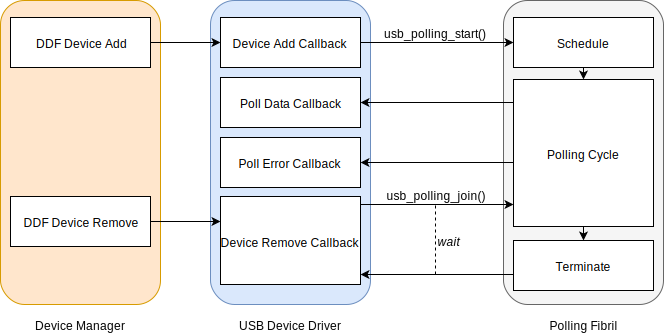
\includegraphics[width=0.8\textwidth]{usb-polling}
	\caption[USB device polling interactions diagram.]{A diagram of interactions
	between the Device Manager, USB device driver and one of its polling fibrils
	during its lifecycle.}
	\label{fig:usb-polling}
\end{figure}

The configuration structure \struct{usb_device_auto_polling_t} has been renamed
for simplicity sake to \struct{usb_polling_t}. Instead of serving as a one-time
configuration structure during polling initiation, its role changed to represent
the entire instance of the polling process throughout its lifetime.

Introducing standard functions such as \fnc{usb_polling_init()} and
\fnc{usb_polling_fini()}, the device driver is now fully responsible for the
ownership of the structure. This is convenient, since drivers often have their
own structures for device data, where \struct{usb_polling_t} can be placed as a
field, dropping the need for additional calls to \fnc{malloc()} and
\fnc{free()}. In addition, this resolves the problem with default values of
various configuration parameters, since in \fnc{usb_polling_init()} all
parameters are assigned their default values and device driver can override only
those desired.

All four of the original polling initialization functions were unified into a
single function \fnc{usb_polling_start()}. Since there is now a clear structure,
which represents the polling instance, the arguments of the original four
functions were moved to \struct{usb_polling_t}, where they are clearly named and
documented, preventing any possible errors from their misinterpretation. Suffice
it to say, that the original four functions mostly fulfilled the role of syntax
sugar, which is now rendered unnecessary, given the fact that default values of
configuration parameters are pre-filled in the polling structure.

Lastly, the API was extended with the \fnc{usb_polling_join()} function, which
closes the polling pipe and consistently waits until the polling fibril
terminates. This function addresses the problem of spinning in driver's
\fnc{device_remove()} or \fnc{device_gone()} callbacks, or possible negligence,
which may result in the polling fibril outliving the device and then accessing
invalid memory. Calling this function in this context will result in the
immediate and synchronous termination of the polling mechanism prior to
deallocation (as depicted in Figure \ref{fig:usb-polling}).

Furthermore, the exposure of internal polling parameters now gives device
drivers more creativity in their approach to polling. For instance, drivers can
now inquire about the state of the polling fibril without the need to have a
private flag maintained by their polling callbacks. The drivers can also change
polling parameters such as request size or polling delay mid-flight, which is a
more flexible approach than to stop polling, change parameters and then start
polling again (note that stopping polling at will was not supported by the
previous implementation without generating actual errors from the hardware
device).

A nice minimalistic example of the new polling mechanism usage can be found in
Listing \ref{lst:polling-example}

\begin{listing}
	\begin{code}
		static usb_polling_t polling;
		static uint8_t buffer[13];

		static bool callback(usb_device_t *dev, uint8_t *buffer, size_t size, void *arg)
		{
			printf("Have data!/n");

			// Return true if we wish to continue polling.
			return true;
		}

		static void demo()
		{
			// Initialize.
			usb_polling_init(&polling);

			// Configure.
			polling.device = /* some usb_device_t here */;
			polling.ep_mapping = /* some interrupt(in) endpoint of the device */;
			polling.buffer = buffer;
			polling.request_size = sizeof(buffer);
			polling.on_data = callback;

			// Start polling.
			usb_polling_start(&polling);

			// Sleep synchronously for a while.
			async_usleep(10000);

			// End polling and clean up.
			usb_polling_join(&polling);
			usb_polling_fini(&polling);
		}
	\end{code}
	\caption{Minimal usage example of the new USB device polling mechanism.}
	\label{lst:polling-example}
\end{listing}

